\documentclass[
	classe=$1^{ere}STI2D$,
]{exercice}

\usepackage{lscape}

\newcommand{\Courbe}[4]{
	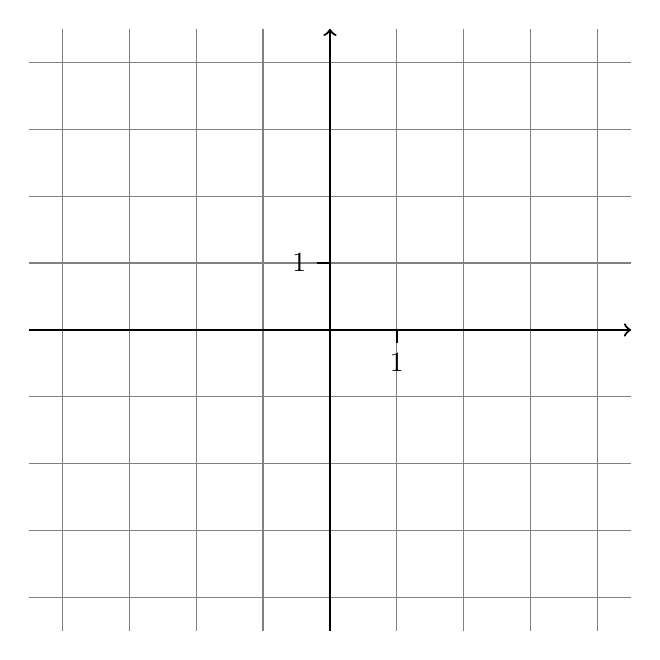
\begin{tikzpicture}[scale=0.85]
		\draw[thin,gray] (-4.5,-4.5) grid (4.5,4.5);
		\draw[thick,->] (-4.5,0) -- (4.5,0);
		\draw[thick,->] (0,-4.5) -- (0,4.5);
		\draw[thick] (1,0) -- ++(0,-0.2) node[below] {$1$};
		\draw[thick] (0,1) -- ++(-0.2,0) node[left] {$1$};

		\ifdefined\makeCorrection
			\draw[variable=\x,domain=-4:4,red] plot({\x},{#1*\x*\x + #2*\x + #3});
		\fi
	\end{tikzpicture}
	\vspace{1em}

	#4
}

\title{Courbes de fonctions de degré 2}

\begin{document}

\maketitle

\newcommand{\Exercice}{
	Tracer le graphe des fonctions suivantes : \medskip

	\begin{minipage}{0.5\textwidth}
		\begin{center}
			\Courbe{1/4}{-1/2}{-2}{$f(x) = \frac{1}{4}x² - \frac{1}{2}x - 2$}
		\end{center}
	\end{minipage}\hfill%
	\begin{minipage}{0.5\textwidth}
		\begin{center}
			\Courbe{-1/2}{0}{4}{$g(x) = -\frac{1}{2}x² + 4$}
		\end{center}
	\end{minipage}
}

\Exercice

\vspace{2cm}

\makebox[\columnwidth]{
	Lycée La Martinière Diderot
	\hfill
	$1^{ere}STI2D$ - Mathématiques
	\hfill
	Exercices
}\vspace{0.105cm}\hrule\vspace{1cm}

\maketitle

\Exercice

\end{document}